%\begin{multicols}{2}
\section{Preliminary Results}
\secsubhead{I apologise for the information density of the figures.
I didn't have time to make simpler ones.}
\label{app:results}

\subsection{How to read the figures}
\label{sec:heatmaps}
%Heatmaps are ubiquitous in bioinformatics for visualizing very large data sets.
In Fig. \ref{fig:E_MNIST} and \ref{fig:K_MNIST}, rows are samples and columns are activations.
Samples are split either by training label (Fig. \ref{fig:E_MNIST}) or predicted label (Fig. \ref{fig:K_MNIST}.
Activations are split by model.
For Fig. \ref{fig:E_MNIST}, these are the encoder activations.
\textsf{bottleneck} gives the bottleneck activations for the outer model.
%\end{multicols}

\begin{figure}{\textwidth}
\centering
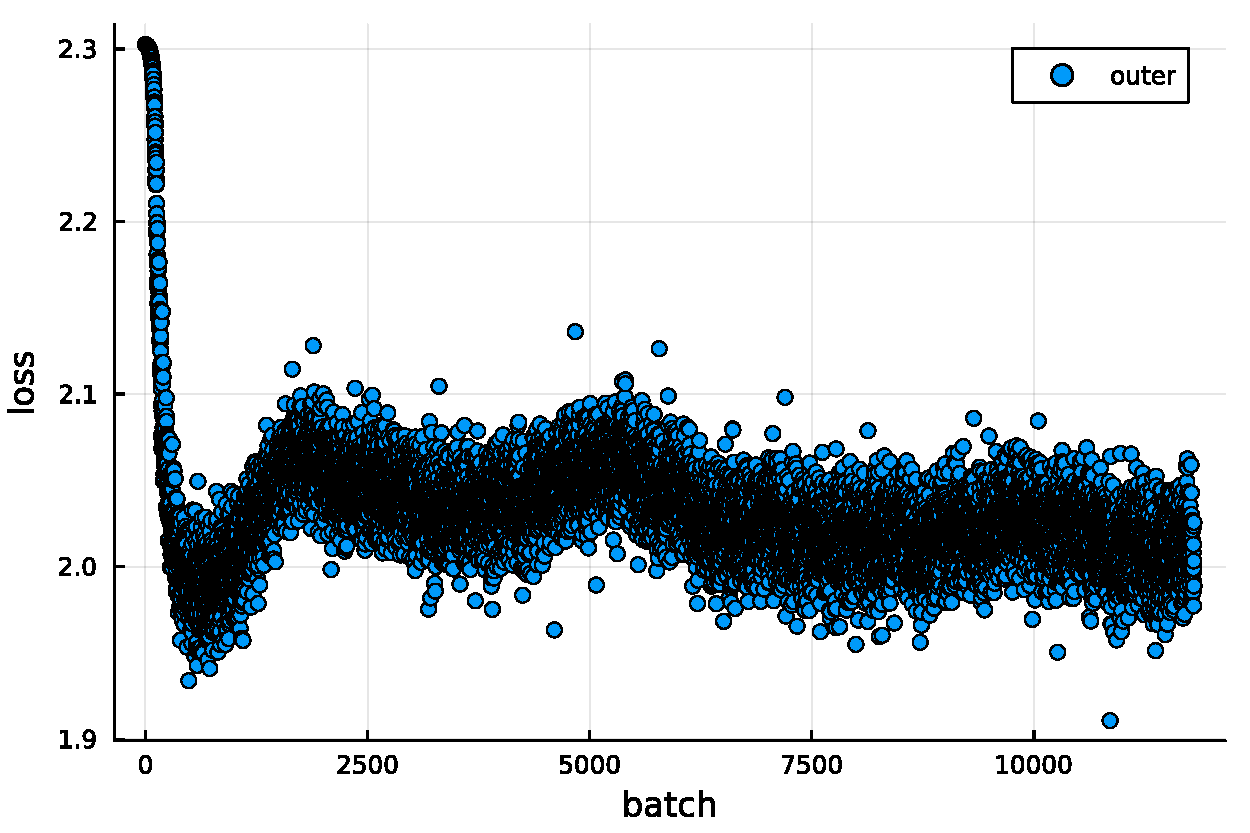
\includegraphics[width=\textwidth]{fig/loss_outer.pdf}
\caption{Outer model loss (logit crossentropy) compared to data labels.}
\label{fig:lossouter}
\end{figure}

\begin{figure}{\textwidth}
    \centering
    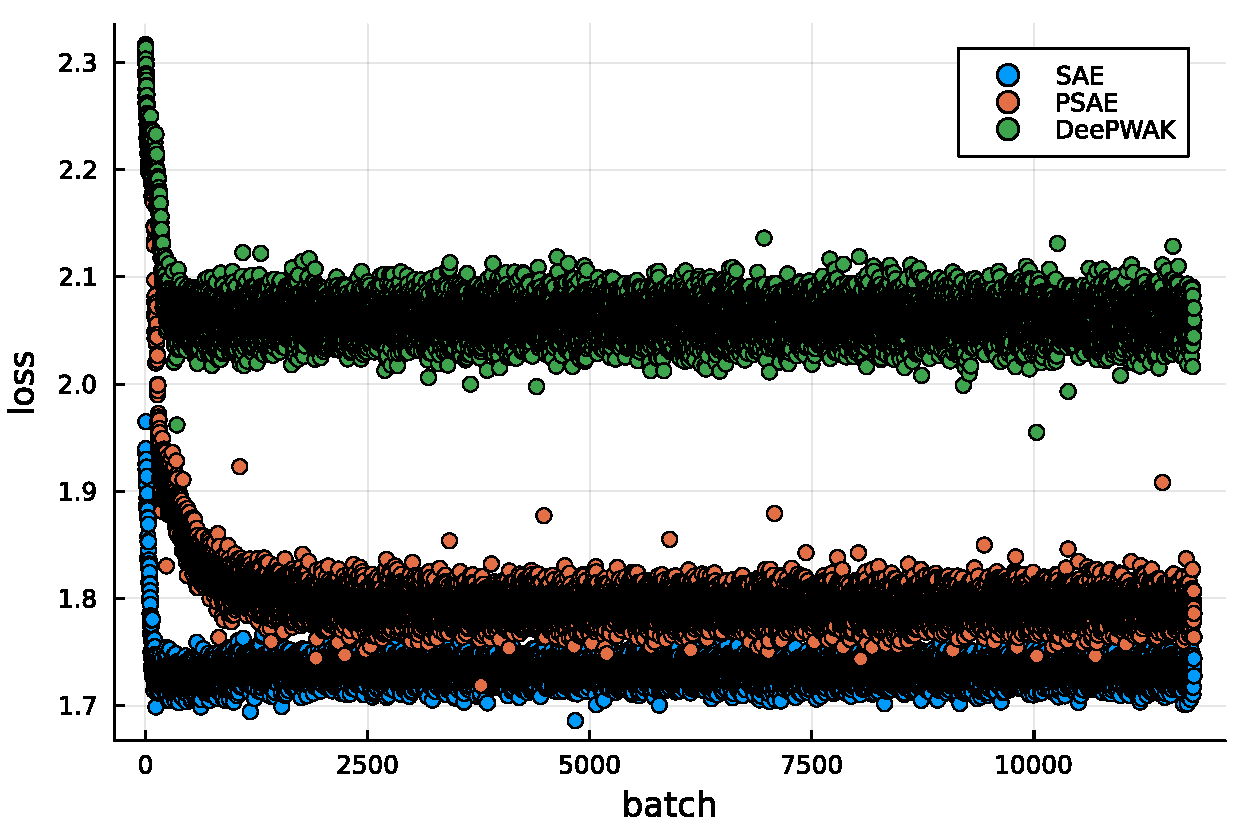
\includegraphics[width=\textwidth]{fig/loss_inner.pdf}
    \caption{Inner model loss (logit crossentropy) compared to the prediction of the outer model.}
    \label{fig:lossinner}
\end{figure}


\begin{figure}
  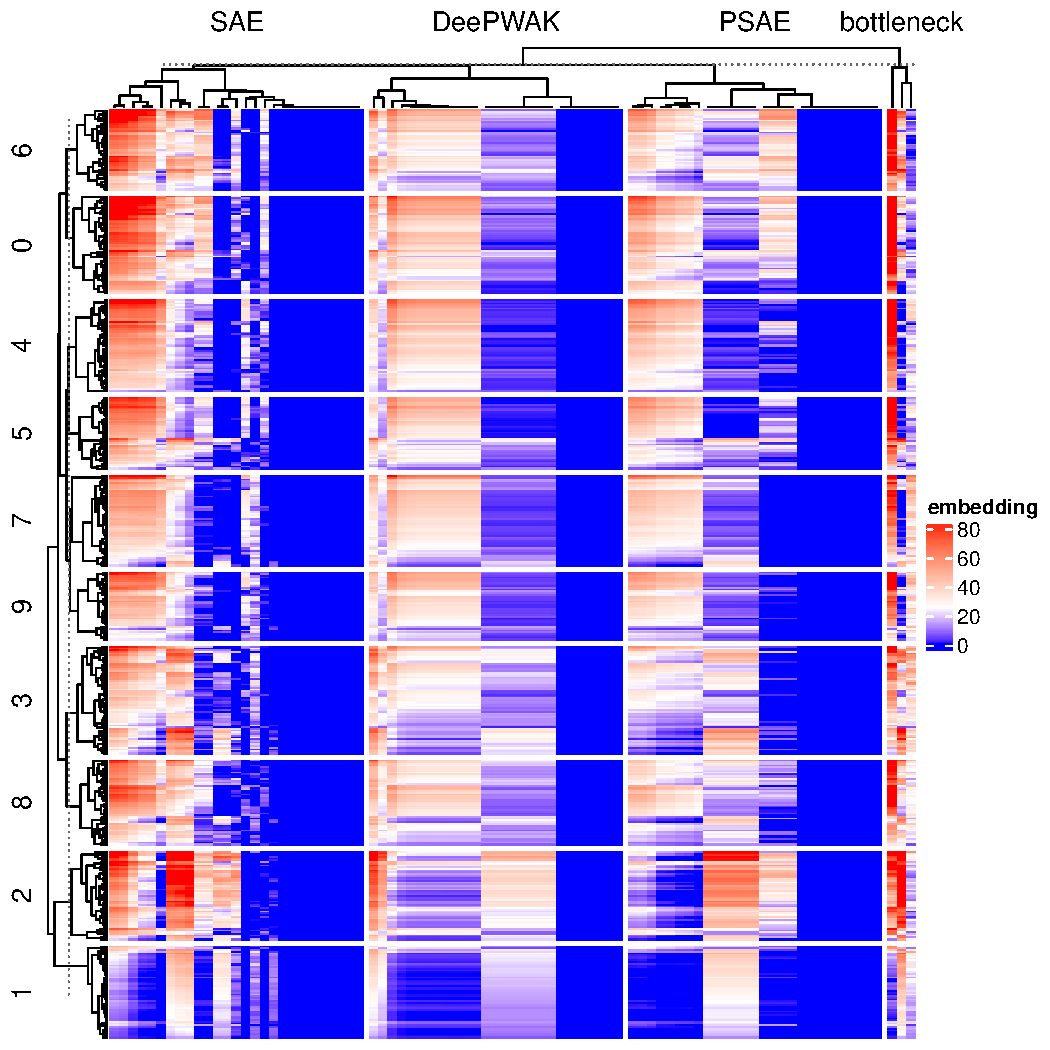
\includegraphics[width=\textwidth]{E_labels.pdf}
  \caption{Feature splitting of bottleneck activations by different methods.
    There is a clear progression of sparcity from a na\"ive SAE, PSAE, and DeePWAK.
    Rows are split by training set label.
    Interestingly, adding a partitioner submodel seems to result in the same feature being copied by multiple embeddings.}
    \label{fig:E_MNIST}
\end{figure}

\begin{figure}
  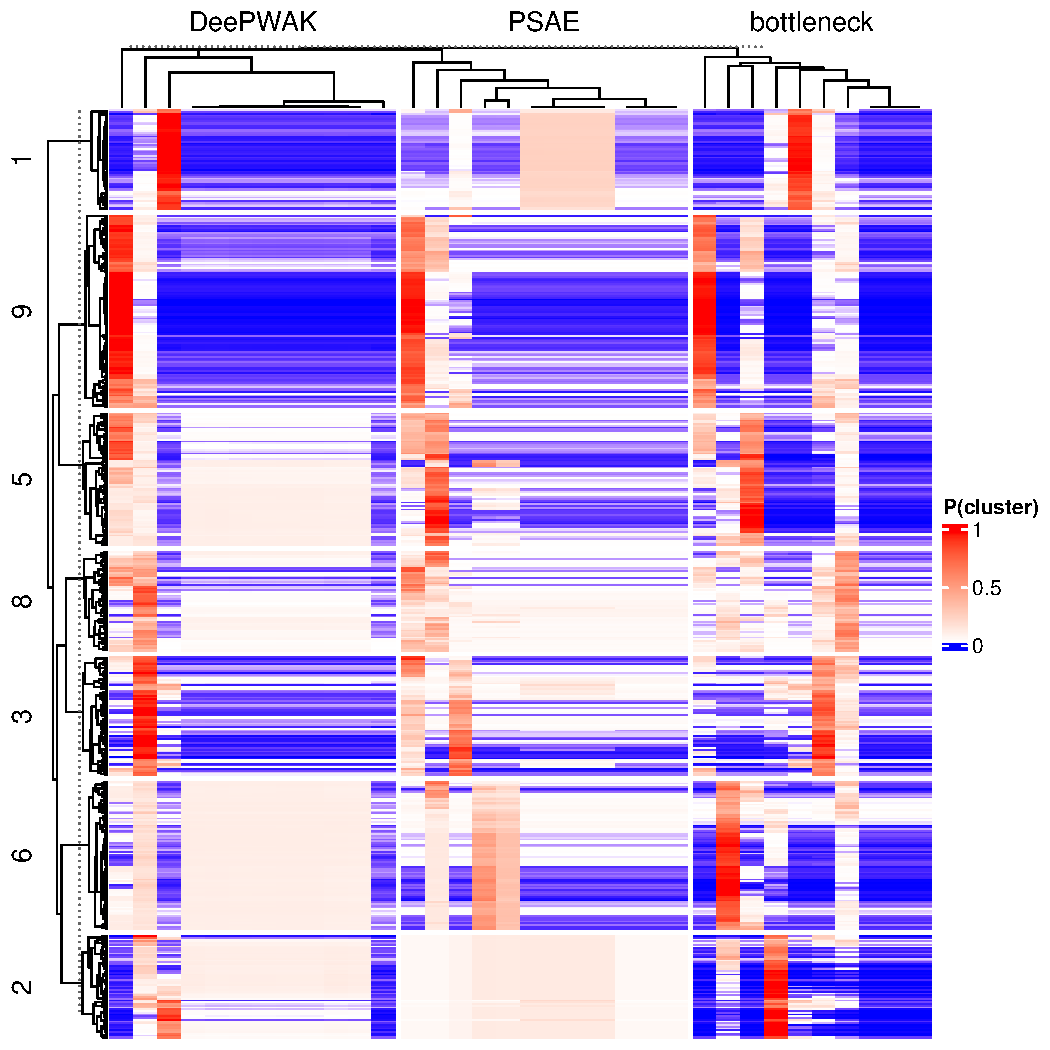
\includegraphics[width=\textwidth]{K_predicted.pdf}
    \caption{Both DeePWAK and PSEA learn sparse clusters. Rows are split by predicted label.}
    \label{fig:K_MNIST}
\end{figure}

\begin{figure}
  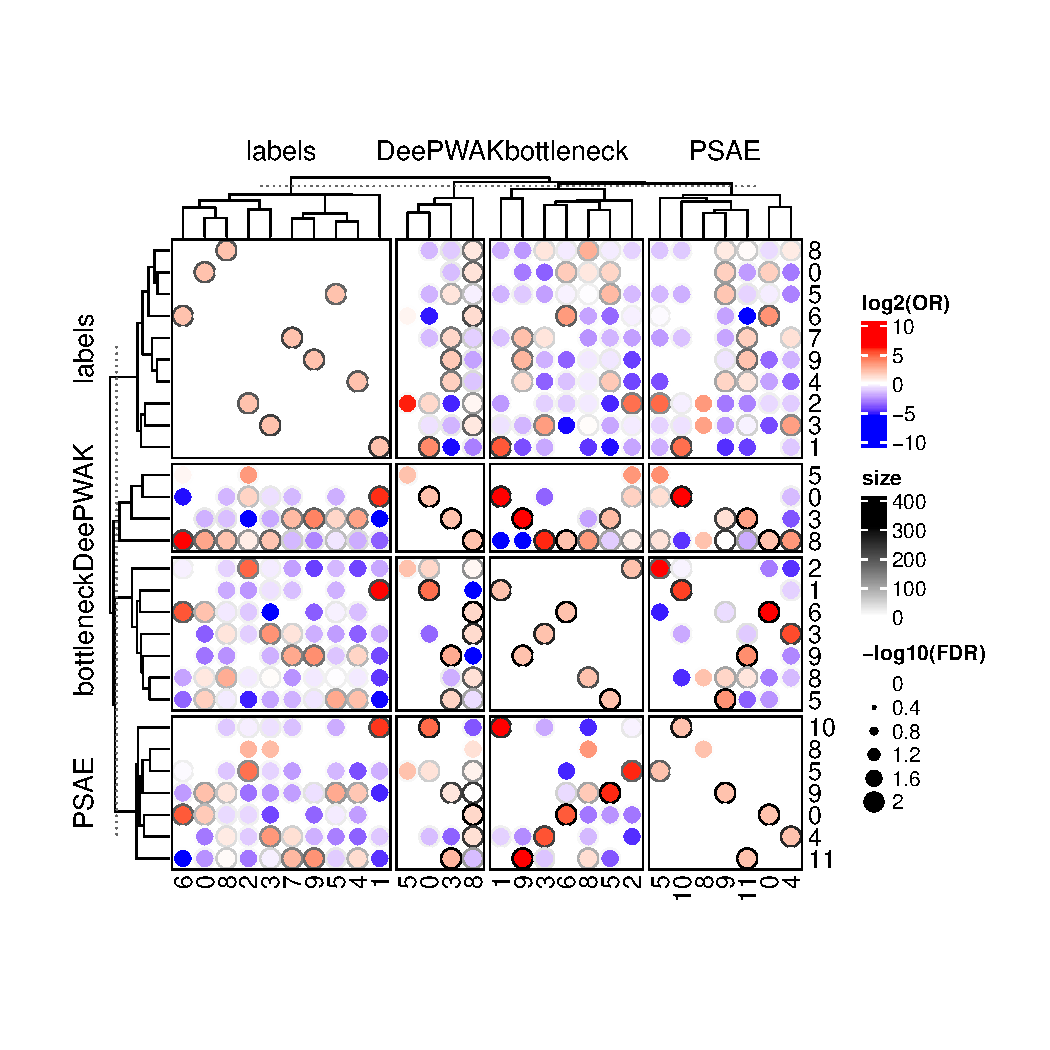
\includegraphics[width=\textwidth]{enrichment.pdf}
    \caption{Hypergeometric test for enrichment of [rows] in [columns].}
    \label{fig:hyperMNIST}
\end{figure}

%\begin{multicols}{2}
    
Even trained without a sparcity correction, \DeePWAK finds a more sparse representation than the SAE or PSAE (Fig. \ref{fig:E_MNIST}, \ref{fig:K_MNIST}.

Both DeePWAK and PSAE seem to capture latent features from the bottleneck (Fig. \ref{fig:hyperMNIST}.
Strikingly, PSAE better predicts the model output than the model predicts the training labels.
DeePWAK, on the other hand, appears to identify higher level features used by the model for classification.
It reveals the model apparently grouping rounded (0,3,6,8) and pointed (4,5,7,9) digits. 
Even more curiously, these features appear \textit{bisemantic}.
Looking at \textsf{DeePWAK 0}, this cluster appears to regard 6 as ``opposite'' of 1.
If we look back at Fig. \ref{fig:K_MNIST}, we can see the partitioner is much less confident classifying 6s than other digits.
It's possible the model is using an internal logic of ``I don't know what this is but it's definitely not a 1''.


